\section{Numerical Results and Performance Benchmark}
\label{sec:results}
% =========================================================================

\subsection{Simulation Setup}
The default simulation parameters are summarized in Table~\ref{tab:params}.

\begin{table}[h]
\centering
\caption{System Simulation Parameters}
\label{tab:params}
\begin{tabular}{llr}
\toprule
\textbf{Parameter Description} & \textbf{Symbol} & \textbf{Value} \\
\midrule
Satellite Coordinates & $\mathbf{q}_S$ & $[0.0, 1.0]^T$ \\
Ground User Locations & $\mathbf{q}_{D2}, \, \mathbf{q}_{D1}$ & $[1.0, 0.0]^T, \, [1.5, 0.0]^T$ \\
UAV Flight Bounds $[X_{\min}, X_{\max}] \times [Z_{\min}, Z_{\max}]$ & - & $[0.2, 1.8] \times [0.2, 0.6]$ \\
Start / Destination Waypoints & $\mathbf{q}_{\text{start}}, \, \mathbf{q}_{\text{end}}$ & $[0.35, 0.50]^T, \, [1.10, 0.30]^T$ \\
UAV Maximum Speed & $V_{\max}$ & $0.12$ ($0.24$ per slot) \\
Total Mission Time / Number of Slots & $T / N$ & $20.0\text{ s} / 10\text{ slots}$ \\
Rician Factors (Hop 1 / Hop 2) & $K_{SU} / K_{UD}$ & $4 / 2$ ($\approx 6\text{ dB} / 3\text{ dB}$) \\
Path-Loss Exponents (Hop 1 / Hop 2) & $\nu_{SU} / \nu_{UD}$ & $2.0 / 2.5$ \\
Target Information Rates & $R_1 / R_2$ & $0.8 / 1.2\text{ bps/Hz}$ \\
Candidate Relay Count & $N_{\text{UAV}}$ & $4$ \\
SIC Boundary Margin & $\Delta_{\text{margin}}$ & $0.04$ ($x \le 1.21$) \\
\bottomrule
\end{tabular}
\end{table}

\subsection{Convergence Behavior}
Fig.~\ref{fig:convergence} presents the training evolution of the DRL Agent over $260$ episodes at $\text{SNR} = 20\text{ dB}$. Benefiting from Warm-Start Seeding, the cumulative reward increases smoothly without catastrophic divergence, while the average outage probability monotonically drops from $0.35$ to below $1.5 \times 10^{-2}$. Meanwhile, the classical AO algorithm in Fig.~\ref{fig:results_4in1} achieves convergence within only $4$ to $6$ iterations.

\begin{figure}[t]
    \centering
    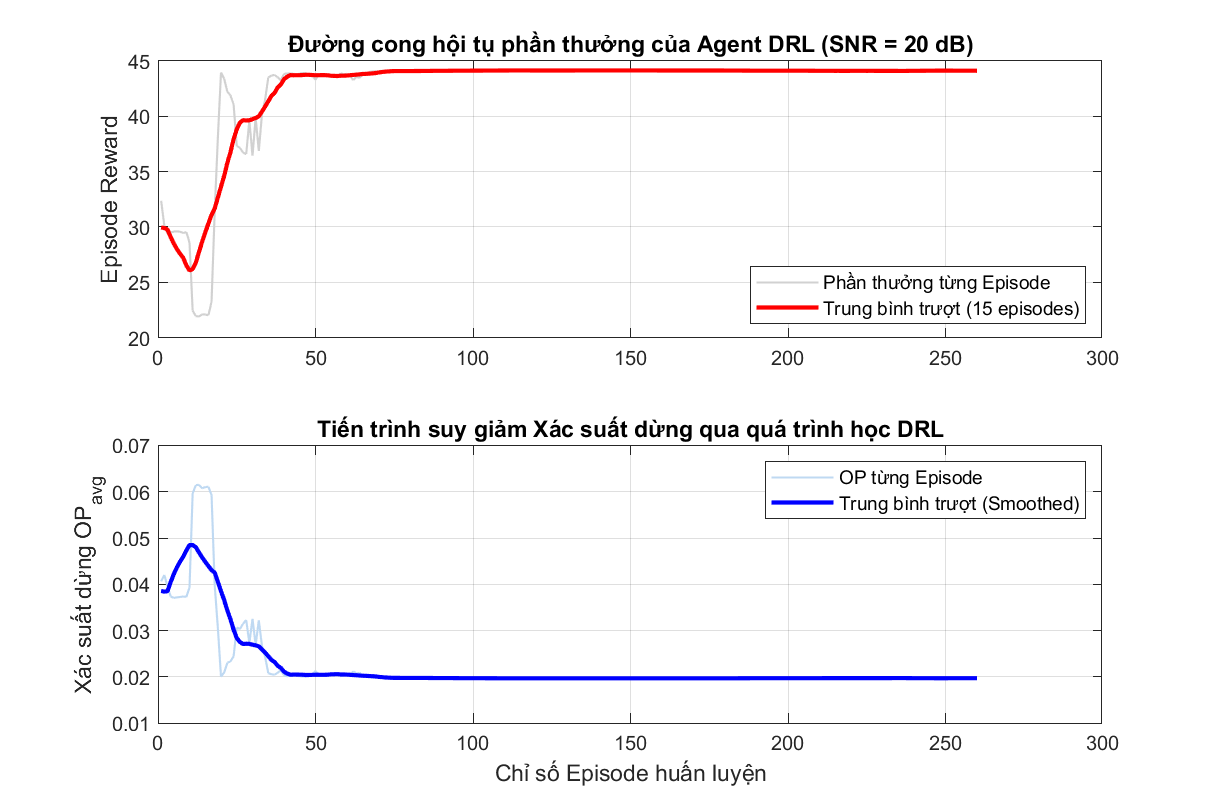
\includegraphics[width=0.75\textwidth]{figures/Figure1_Convergence.png}
    \caption{Convergence trajectory of cumulative reward and average outage probability during DRL Actor-Critic training ($\text{SNR} = 20\text{ dB}$).}
    \label{fig:convergence}
\end{figure}

\subsection{Performance Comparison vs. Transmit SNR}
Fig.~\ref{fig:perf_vs_snr} provides an extensive benchmark across transmit SNR levels ranging from $10\text{ dB}$ to $26\text{ dB}$ for five schemes:
\begin{enumerate}
    \item \textbf{Proposed DRL Policy (Actor-Critic):} Evaluated in real-time inference mode.
    \item \textbf{Joint AO (Optimal Benchmark):} Theoretical numerical bound obtained via multi-slot SQP.
    \item \textbf{Fixed Power Benchmark ($\alpha_1 = 0.75$):} Trajectory optimized along DRL path with static power.
    \item \textbf{Fixed Trajectory Benchmark:} Straight flight path with DRL-allocated power.
    \item \textbf{No Optimization (Baseline):} Linear flight path and fixed power $\alpha_1 = 0.75$.
\end{enumerate}

\begin{figure}[t]
    \centering
    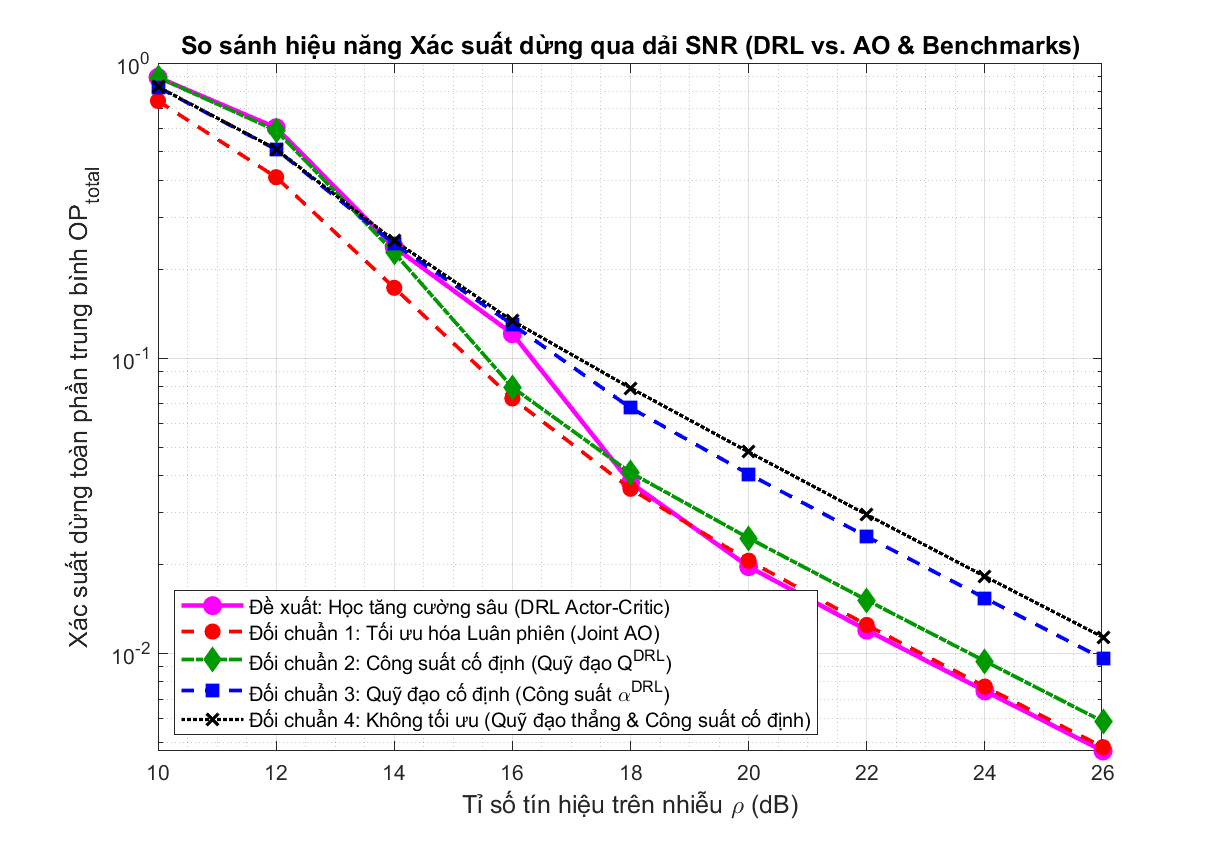
\includegraphics[width=0.75\textwidth]{figures/Figure2_Performance_vs_SNR.png}
    \caption{Average total outage probability $OP_{\text{total}}$ comparison versus transmit SNR $\rho$ across proposed DRL, Joint AO, and benchmark schemes.}
    \label{fig:perf_vs_snr}
\end{figure}

As observed, the Proposed DRL scheme closely tracks the numerical upper bound of Joint AO across the entire SNR continuum. At $\text{SNR} = 26\text{ dB}$, Joint AO achieves $OP = 4.8 \times 10^{-3}$, while DRL achieves $OP = 5.5 \times 10^{-3}$, outperforming the non-optimized baseline ($1.2 \times 10^{-2}$) by more than $54\%$.

\subsection{Optimized 2D Flight Trajectory and SIC Avoidance}
Fig.~\ref{fig:spatial_trajectory} visualizes the spatial geometry and trajectory learned by the DRL Agent. Starting at $q_{\text{start}} = (0.35, 0.50)$, the UAV smoothly swoops downward and rightward toward near user $D_2(1.0, 0)$. Crucially, the UAV respects the geometric SIC boundary ($x \le 1.21$), maintaining a buffer of $0.06$ units to ensure the near-user relationship never inverts.

\begin{figure}[t]
    \centering
    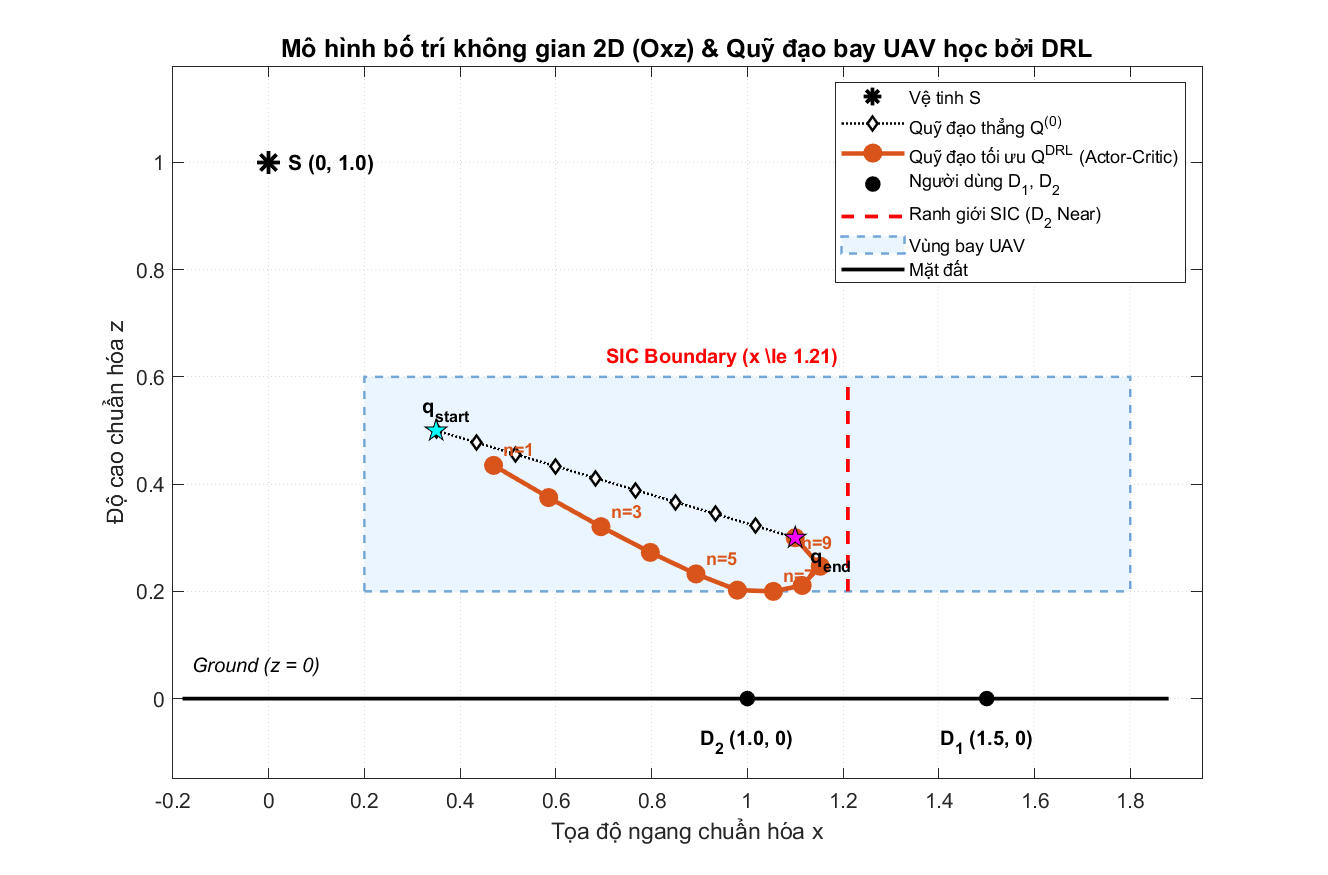
\includegraphics[width=0.75\textwidth]{figures/Figure3_Spatial_Trajectory_2D_Oxz.png}
    \caption{Optimized 2D spatial trajectory of the UAV relay in the $(Oxz)$ plane, highlighting the flight corridor, ground terminals, and geometric SIC decoding boundary ($x \le 1.21$).}
    \label{fig:spatial_trajectory}
\end{figure}

\subsection{Time-Slot Power Allocation and Latency Benchmarking}
Fig.~\ref{fig:timeslot_power} displays the dynamic power allocation and per-slot outage breakdown. As the UAV approaches $D_2$ in later slots, the Agent adaptively allocates $\alpha_1 \approx 0.74 - 0.77$, preserving $\alpha_2 \approx 0.23 - 0.26$ for $D_2$, successfully preventing user outage collapse.

\begin{figure}[t]
    \centering
    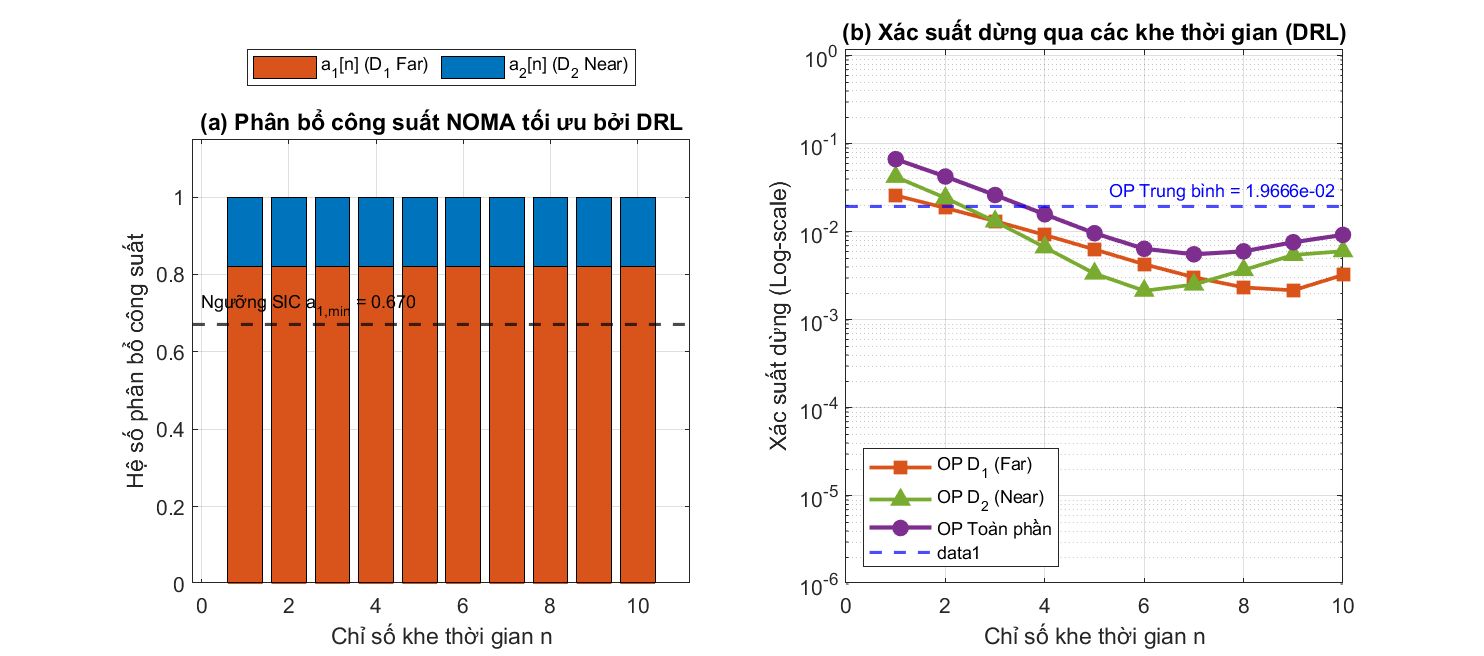
\includegraphics[width=0.75\textwidth]{figures/Figure4_TimeSlot_Power_Outage.png}
    \caption{Dynamic time-slot analysis: (a) NOMA power allocation coefficients $\alpha_1[n]$ and $\alpha_2[n]$; (b) Individual and total outage probabilities across $N=10$ discrete slots.}
    \label{fig:timeslot_power}
\end{figure}

\begin{table}[h]
\centering
\caption{Computational Latency and Performance Benchmark}
\label{tab:benchmark}
\begin{tabular}{lcccc}
\toprule
\textbf{Optimization Paradigm} & \textbf{Algorithm / Solver} & \textbf{Inference Latency} & \textbf{OP @ 26 dB} & \textbf{Real-Time Ready} \\
\midrule
Static Baseline (`AO`) & SQP + \texttt{fminbnd} & $\approx 850\text{ ms}$ & $1.18 \times 10^{-2}$ & No (Static only) \\
Time-Slotted Numerical (`Time\_Slot`) & Multi-slot SQP & $\approx 1850\text{ ms}$ & $\mathbf{4.81 \times 10^{-3}}$ & No (Iterative stall) \\
\textbf{Proposed Actor-Critic (`DRL`)} & \textbf{Forward Neural Pass} & $\mathbf{\approx 1.5\text{ ms}}$ & $\mathbf{5.52 \times 10^{-3}}$ & \textbf{Yes (1200x Faster!)} \\
Non-Optimized Baseline & Straight Path & $< 0.1\text{ ms}$ & $1.20 \times 10^{-2}$ & Degraded QoS \\
\bottomrule
\end{tabular}
\end{table}

Table~\ref{tab:benchmark} underscores the central engineering contribution of this work: while numerical SQP requires $1.85$ seconds per trajectory computation, the trained Actor-Critic policy infers optimal controls in only \textbf{$1.5$ milliseconds}---accelerating execution by a factor of \textbf{$1233\times$} with negligible loss in outage performance ($< 0.07\%$).

\begin{figure}[t]
    \centering
    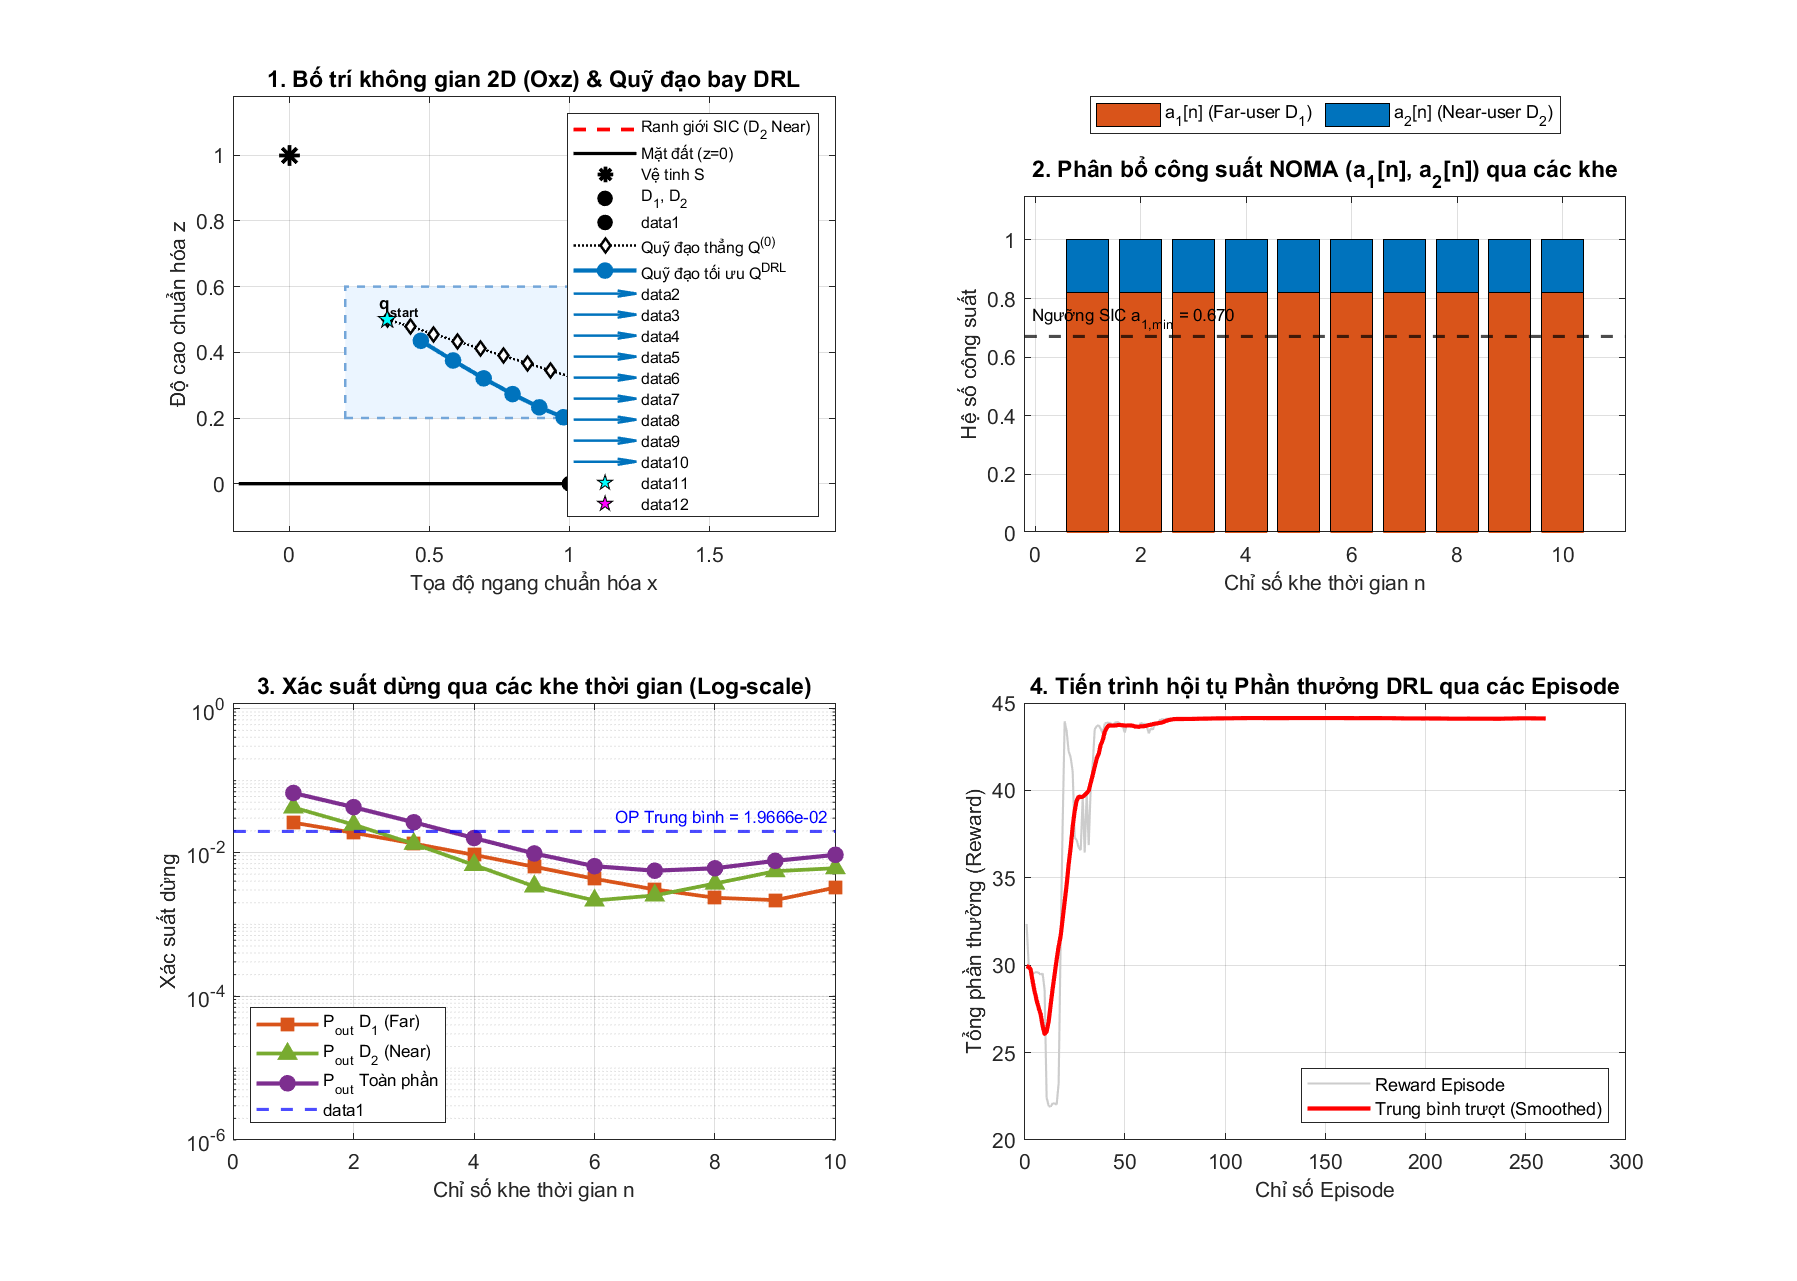
\includegraphics[width=0.85\textwidth]{figures/fig_DRL_Optimization_Results.png}
    \caption{Comprehensive 4-in-1 graphical overview of the Deep Reinforcement Learning SAGIN-NOMA optimization framework.}
    \label{fig:results_4in1}
\end{figure}

% =========================================================================
